\documentclass{beamer}
\usepackage[utf8]{inputenc}

\usetheme{Madrid}
\usecolortheme{default}
\usepackage{amsmath,amssymb,amsfonts,amsthm}
\usepackage{txfonts}
\usepackage{tkz-euclide}
\usepackage{listings}
\usepackage{adjustbox}
\usepackage{array}
\usepackage{tabularx}
\usepackage{gvv}
\usepackage{lmodern}
\usepackage{circuitikz}
\usepackage{tikz}
\usepackage{graphicx}

\setbeamertemplate{page number in head/foot}[totalframenumber]

\usepackage{tcolorbox}
\tcbuselibrary{minted,breakable,xparse,skins}



\definecolor{bg}{gray}{0.95}
\DeclareTCBListing{mintedbox}{O{}m!O{}}{%
  breakable=true,
  listing engine=minted,
  listing only,
  minted language=#2,
  minted style=default,
  minted options={%
    linenos,
    gobble=0,
    breaklines=true,
    breakafter=,,
    fontsize=\small,
    numbersep=8pt,
    #1},
  boxsep=0pt,
  left skip=0pt,
  right skip=0pt,
  left=25pt,
  right=0pt,
  top=3pt,
  bottom=3pt,
  arc=5pt,
  leftrule=0pt,
  rightrule=0pt,
  bottomrule=2pt,
  toprule=2pt,
  colback=bg,
  colframe=orange!70,
  enhanced,
  overlay={%
    \begin{tcbclipinterior}
    \fill[orange!20!white] (frame.south west) rectangle ([xshift=20pt]frame.north west);
    \end{tcbclipinterior}},
  #3,
}
\lstset{
    language=C,
    basicstyle=\ttfamily\small,
    keywordstyle=\color{blue},
    stringstyle=\color{orange},
    commentstyle=\color{green!60!black},
    numbers=left,
    numberstyle=\tiny\color{gray},
    breaklines=true,
    showstringspaces=false,
}
%------------------------------------------------------------

\title
{4.7.64}
\date{September 4,2025}
\author 
{AI25BTECH11003 - Bhavesh Gaikwad}



\begin{document}


\frame{\titlepage}
\begin{frame}{Question}
\centering
Find the distance between the point $\vec{P}$(6, 5, 9) and the plane determined by the points $\vec{A}$(3, -1, 2), $\vec{B}$(5, 2, 4) and $\vec{C}$(-1, -1, 6).
\end{frame}


\begin{frame}[fragile]
    \frametitle{Theoretical Solution}
Given:
\begin{equation}
\vec{P} = \myvec{6 \\ 5 \\ 9}, \, \vec{A} = \myvec{3 \\ -1 \\ 2}, \, \vec{B} = \myvec{5 \\ 2 \\ 4}, \, \vec{C} = \myvec{-1 \\ -1 \\ 6}
\end{equation}\\
Let $\vec{n}$ be the perpendicular vector to plane.

\begin{equation}
    \vec{n} = \vec{(B-A)} \times \vec{(C-A)} = \myvec{|\vec{A_{23}} & \vec{B_{23}}| \\ |\vec{A_{31}} & \vec{B_{31}}| \\ |\vec{A_{12}} & \vec{B_{12}}|} = \myvec{12 \\ -16 \\ 12}
\end{equation}\\

\begin{center}
    OR
\end{center}

\begin{equation}
\vec{n} = \myvec{3 \\ -4 \\ 3}
\end{equation}\\

\end{frame}

\begin{frame}[fragile]
\frametitle{Theoretical Solution}
if $\vec{n} = \myvec{\alpha \\ \beta \\ \gamma}$ then the equation of the plane would be
\begin{equation}
    \alpha(x) + \beta(y) + \gamma(z) = k \text{, Where k is a constant}
\end{equation}\\

From Equation 3 and 4, 
\begin{equation}
    \alpha = 3, \, \beta = -4, \, \gamma = 3
\end{equation}

\begin{equation}
\therefore
\text{ The equation of the plane will be } 3x-4y+3z = k.
\end{equation}


Putting Coordinates of $\vec{A}$ in equation 6 to get k,
\begin{equation}
    k=3(3) - 4(-1) + 3(2) \quad \Rightarrow k= 19
\end{equation}

\begin{equation}
\therefore \, 3x-4y+3z=19
\end{equation}
\end{frame}


\begin{frame}[fragile]
    \frametitle{Theoretical Solution}
    Let $\vec{L}$ be the line perpendicular to plane and passing through $\vec{P}$.\\
Let $\vec{Q}$ be a position vector of a point on the plane and the line $\vec{L}$

\begin{equation}
\text{From Equation 3, } \Rightarrow 
\vec{L} = \vec{P} + t\vec{n}
\quad \Rightarrow \vec{L} = \myvec{6 \\ 5 \\ 9} + t\myvec{3 \\ -4 \\ 3}
\end{equation}


Therefore from Equation 9,
$\vec{Q} = \myvec{6+3t \\ 5-4t \\ 9+3t}$

Putting co-ordinates of $\vec{Q}$ in equation of plane (from equation 8).

\begin{equation}
    3(6+3t) - 4(5-4t) + 3(9+3t) = 19 \quad \Rightarrow t=-\dfrac{3}{17}  
\end{equation}

\begin{equation}
    \therefore \, \vec{Q}=\myvec{93/17 \\ 97/17 \\ 144/17}
\end{equation}
\end{frame}

\begin{frame}[fragile]
    \frametitle{Theoretical Solution}
The Distance between the plane and $\vec{P}$ is $\norm{\vec{P} - \vec{Q}}$
\begin{equation}
\norm{\vec{P} - \vec{Q}}= \norm{\myvec{9/17 \\ -12/17 \\ 9/17}} = \dfrac{3\sqrt{34}}{17}
\end{equation}\\\\


\begin{align}
    \boxed{\text{The Distance between the Plane and } \vec{P} \, is \, \dfrac{3\sqrt{34}}{17} \, units.}
\end{align}
\end{frame}

\begin{frame}[fragile]
    \frametitle{C Code}
    \begin{lstlisting}
#include <stdio.h>
#include <math.h>

/* 3D point and vector types */
typedef struct { double x, y, z; } Point3D;
typedef struct { double x, y, z; } Vector3D;

/* Subtract two points (p1 - p2) -> vector */
Vector3D subtract_points(Point3D p1, Point3D p2) {
    Vector3D r;
    r.x = p1.x - p2.x;
    r.y = p1.y - p2.y;
    r.z = p1.z - p2.z;
    return r;
}
    \end{lstlisting}
\end{frame}

\begin{frame}[fragile]
    \frametitle{C Code}
    \begin{lstlisting}

/* Cross product v1 × v2 */
Vector3D cross_product(Vector3D v1, Vector3D v2) {
    Vector3D r;
    r.x = v1.y * v2.z - v1.z * v2.y;
    r.y = v1.z * v2.x - v1.x * v2.z;
    r.z = v1.x * v2.y - v1.y * v2.x;
    return r;
}

/* Vector magnitude */
double magnitude(Vector3D v) {
    return sqrt(v.x * v.x + v.y * v.y + v.z * v.z);
}
    \end{lstlisting}
\end{frame}

\begin{frame}[fragile]
    \frametitle{C Code}
    \begin{lstlisting}
/* Plane normal from three points: n = (B - A) × (C - A) */
Vector3D find_plane_normal(Point3D A, Point3D B, Point3D C) {
    Vector3D AB = subtract_points(B, A);
    Vector3D AC = subtract_points(C, A);
    return cross_product(AB, AC);
}

/* Plane constant k in: n.x*x + n.y*y + n.z*z = k, using a point on plane */
double find_plane_constant(Point3D A, Vector3D n) {
    return n.x * A.x + n.y * A.y + n.z * A.z;
}
    \end{lstlisting}
\end{frame}

\begin{frame}[fragile]
    \frametitle{C Code}
    \begin{lstlisting}
/* Foot of perpendicular from P to plane with normal n and constant k */
Point3D find_foot_of_perpendicular(Point3D P, Vector3D n, double k) {
    /* Line: L(t) = P + t n; impose n · L(t) = k to solve for t */
    double num = k - (n.x * P.x + n.y * P.y + n.z * P.z);
    double den = n.x * n.x + n.y * n.y + n.z * n.z;
    double t = num / den;

    Point3D Q;
    Q.x = P.x + t * n.x;
    Q.y = P.y + t * n.y;
    Q.z = P.z + t * n.z;
    return Q;
}

    \end{lstlisting}
\end{frame}

\begin{frame}[fragile]
    \frametitle{C Code}
    \begin{lstlisting}

/* Distance between two points */
double distance_between_points(Point3D p1, Point3D p2) {
    Vector3D d = subtract_points(p1, p2);
    return magnitude(d);
}

/* Save points to points.dat in text format */
void save_points_to_file(Point3D A, Point3D B, Point3D C, Point3D P, Point3D Q) {
    FILE *fp = fopen("points.dat", "w");
    if (!fp) return;
    fprintf(fp, "A %.10f %.10f %.10f\n", A.x, A.y, A.z);
    fprintf(fp, "B %.10f %.10f %.10f\n", B.x, B.y, B.z);
    fprintf(fp, "C %.10f %.10f %.10f\n", C.x, C.y, C.z);
    fprintf(fp, "P %.10f %.10f %.10f\n", P.x, P.y, P.z);
    fprintf(fp, "Q %.10f %.10f %.10f\n", Q.x, Q.y, Q.z);
    fclose(fp);
}
    \end{lstlisting}
\end{frame}

\begin{frame}[fragile]
    \frametitle{C Code}
    \begin{lstlisting}
/* Solve distance from P to plane ABC, return distance, write Q via pointer, and save A,B,C,P,Q to points.dat */
double solve_point_to_plane_distance(Point3D A, Point3D B, Point3D C, Point3D P, Point3D *Q_out) {
    Vector3D n = find_plane_normal(A, B, C);
    double k = find_plane_constant(A, n);
    Point3D Q = find_foot_of_perpendicular(P, n, k);
    if (Q_out) *Q_out = Q;
    save_points_to_file(A, B, C, P, Q);
    return distance_between_points(P, Q);
}
    \end{lstlisting}
\end{frame}

\begin{frame}[fragile]
    \frametitle{C Code}
    \begin{lstlisting}
/* Convenience function with the exact problem data from the PDF:
   A(3,-1,2), B(5,2,4), C(-1,-1,6), P(6,5,9).
   Calls the solver, writes points.dat, and returns the distance. */
double generate_points_and_save(void) {
    Point3D A = { 3.0, -1.0, 2.0 };
    Point3D B = { 5.0,  2.0, 4.0 };
    Point3D C = {-1.0, -1.0, 6.0 };
    Point3D P = { 6.0,  5.0, 9.0 };
    Point3D Q;
    return solve_point_to_plane_distance(A, B, C, P, &Q);
}
    \end{lstlisting}
\end{frame}

\begin{frame}[fragile]
    \frametitle{Python Code}
    \begin{lstlisting}
import ctypes
import numpy as np
import matplotlib.pyplot as plt
from mpl_toolkits.mplot3d import Axes3D
import os

# Load the shared library
lib = ctypes.CDLL('./plane.so')

# Define the Point3D structure for ctypes
class Point3D(ctypes.Structure):
    _fields_ = [("x", ctypes.c_double),
                ("y", ctypes.c_double), 
                ("z", ctypes.c_double)]
    \end{lstlisting}
\end{frame}

\begin{frame}[fragile]
    \frametitle{Python Code}
    \begin{lstlisting}
class Vector3D(ctypes.Structure):
    _fields_ = [("x", ctypes.c_double),
                ("y", ctypes.c_double),
                ("z", ctypes.c_double)]

# Define function signatures
lib.solve_point_to_plane_distance.argtypes = [Point3D, Point3D, Point3D, Point3D, ctypes.POINTER(Point3D)]
lib.solve_point_to_plane_distance.restype = ctypes.c_double

def read_points_from_file(filename):
    """Read points from the data file"""
    points = {}
    \end{lstlisting}
\end{frame}

\begin{frame}[fragile]
    \frametitle{Python Code}
    \begin{lstlisting}
if not os.path.exists(filename):
        print(f"File {filename} not found. Running C program first...")
        # If points.dat doesn't exist, we need to run the C program
        os.system('make main')

    with open(filename, 'r') as f:
        for line in f:
            parts = line.strip().split()
            if len(parts) == 4:
                label = parts[0]
                x, y, z = map(float, parts[1:])
                points[label] = (x, y, z)

    return points
    \end{lstlisting}
\end{frame}

\begin{frame}[fragile]
    \frametitle{Python Code}
    \begin{lstlisting}
def create_visualization(points):
    """Create 3D visualization of points and plane"""
    fig = plt.figure(figsize=(12, 10))
    ax = fig.add_subplot(111, projection='3d')

    # Extract point coordinates
    A = np.array(points['A'])
    B = np.array(points['B'])
    C = np.array(points['C'])
    P = np.array(points['P'])
    Q = np.array(points['Q'])
    \end{lstlisting}
\end{frame}

\begin{frame}[fragile]
    \frametitle{Python Code}
    \begin{lstlisting}
    # Plot the points
    ax.scatter(*A, color='red', s=100, label='A(3,-1,2)')
    ax.scatter(*B, color='green', s=100, label='B(5,2,4)')
    ax.scatter(*C, color='blue', s=100, label='C(-1,-1,6)')
    ax.scatter(*P, color='orange', s=150, label='P(6,5,9)', marker='^')
    ax.scatter(*Q, color='purple', s=120, label='Q (foot of perpendicular)', marker='s')

    # Add text labels for points
    ax.text(A[0], A[1], A[2], '  A', fontsize=12)
    ax.text(B[0], B[1], B[2], '  B', fontsize=12)
    ax.text(C[0], C[1], C[2], '  C', fontsize=12)
    ax.text(P[0], P[1], P[2], '  P', fontsize=12)
    ax.text(Q[0], Q[1], Q[2], '  Q', fontsize=12)
    \end{lstlisting}
\end{frame}

\begin{frame}[fragile]
    \frametitle{Python Code}
    \begin{lstlisting}
# Draw line from P to Q (perpendicular distance)
    ax.plot([P[0], Q[0]], [P[1], Q[1]], [P[2], Q[2]], 'k--', linewidth=2, label='Perpendicular distance')
    
    # Create a grid around the points
    all_points = np.array([A, B, C, P, Q])
    x_min, x_max = all_points[:, 0].min() - 2, all_points[:, 0].max() + 2
    y_min, y_max = all_points[:, 1].min() - 2, all_points[:, 1].max() + 2

    xx, yy = np.meshgrid(np.linspace(x_min, x_max, 20), np.linspace(y_min, y_max, 20))
    zz = (19 - 3*xx + 4*yy) / 3

    # Plot the plane
    ax.plot_surface(xx, yy, zz, alpha=0.3, color='lightblue')
    \end{lstlisting}
\end{frame}

\begin{frame}[fragile]
    \frametitle{Python Code}
    \begin{lstlisting}
# Draw triangle ABC on the plane to show the plane boundary
    triangle_x = [A[0], B[0], C[0], A[0]]
    triangle_y = [A[1], B[1], C[1], A[1]]
    triangle_z = [A[2], B[2], C[2], A[2]]
    ax.plot(triangle_x, triangle_y, triangle_z, 'r-', linewidth=2, label='Triangle ABC')

    # Set labels and title
    ax.set_xlabel('X')
    ax.set_ylabel('Y')
    ax.set_zlabel('Z')
    ax.set_title('4.7.64')
    ax.legend()

    # Set equal aspect ratio
    ax.set_box_aspect([1,1,1])
    \end{lstlisting}
\end{frame}

\begin{frame}[fragile]
    \frametitle{Python Code}
    \begin{lstlisting}
# Save the figure
    plt.tight_layout()
    plt.savefig('fig1.png', dpi=300, bbox_inches='tight')
    plt.close()

    print("Visualization saved as fig1.png")

def main():
    """Main function"""
    # Define the points from the problem
    A = Point3D(3.0, -1.0, 2.0)
    B = Point3D(5.0, 2.0, 4.0)
    C = Point3D(-1.0, -1.0, 6.0)
    P = Point3D(6.0, 5.0, 9.0)
    Q = Point3D()
    \end{lstlisting}
\end{frame}

\begin{frame}[fragile]
    \frametitle{Python Code}
    \begin{lstlisting}
 print("Using shared library to solve the problem...")
    print("Points:")
    print(f"A = ({A.x}, {A.y}, {A.z})")
    print(f"B = ({B.x}, {B.y}, {B.z})")
    print(f"C = ({C.x}, {C.y}, {C.z})")
    print(f"P = ({P.x}, {P.y}, {P.z})")

    try:
        # Call the C function
        distance = lib.solve_point_to_plane_distance(A, B, C, P, ctypes.byref(Q))
        print(f"\nCalculated distance: {distance:.6f} units")
        print(f"Foot of perpendicular Q: ({Q.x:.6f}, {Q.y:.6f}, {Q.z:.6f})")

        # Read points from file and create visualization
        points_dict = read_points_from_file('points.dat')
        print(f"\nPoints read from file: {points_dict}")
    \end{lstlisting}
\end{frame}

\begin{frame}[fragile]
    \frametitle{Python Code}
    \begin{lstlisting}
create_visualization(points_dict)

    except Exception as e:
        print(f"Error: {e}")
        print("Make sure to compile the shared library first with: make plane.so")

if __name__ == "__main__":
    main()
    \end{lstlisting}
\end{frame}

\begin{frame}{Plane}
   \centering
    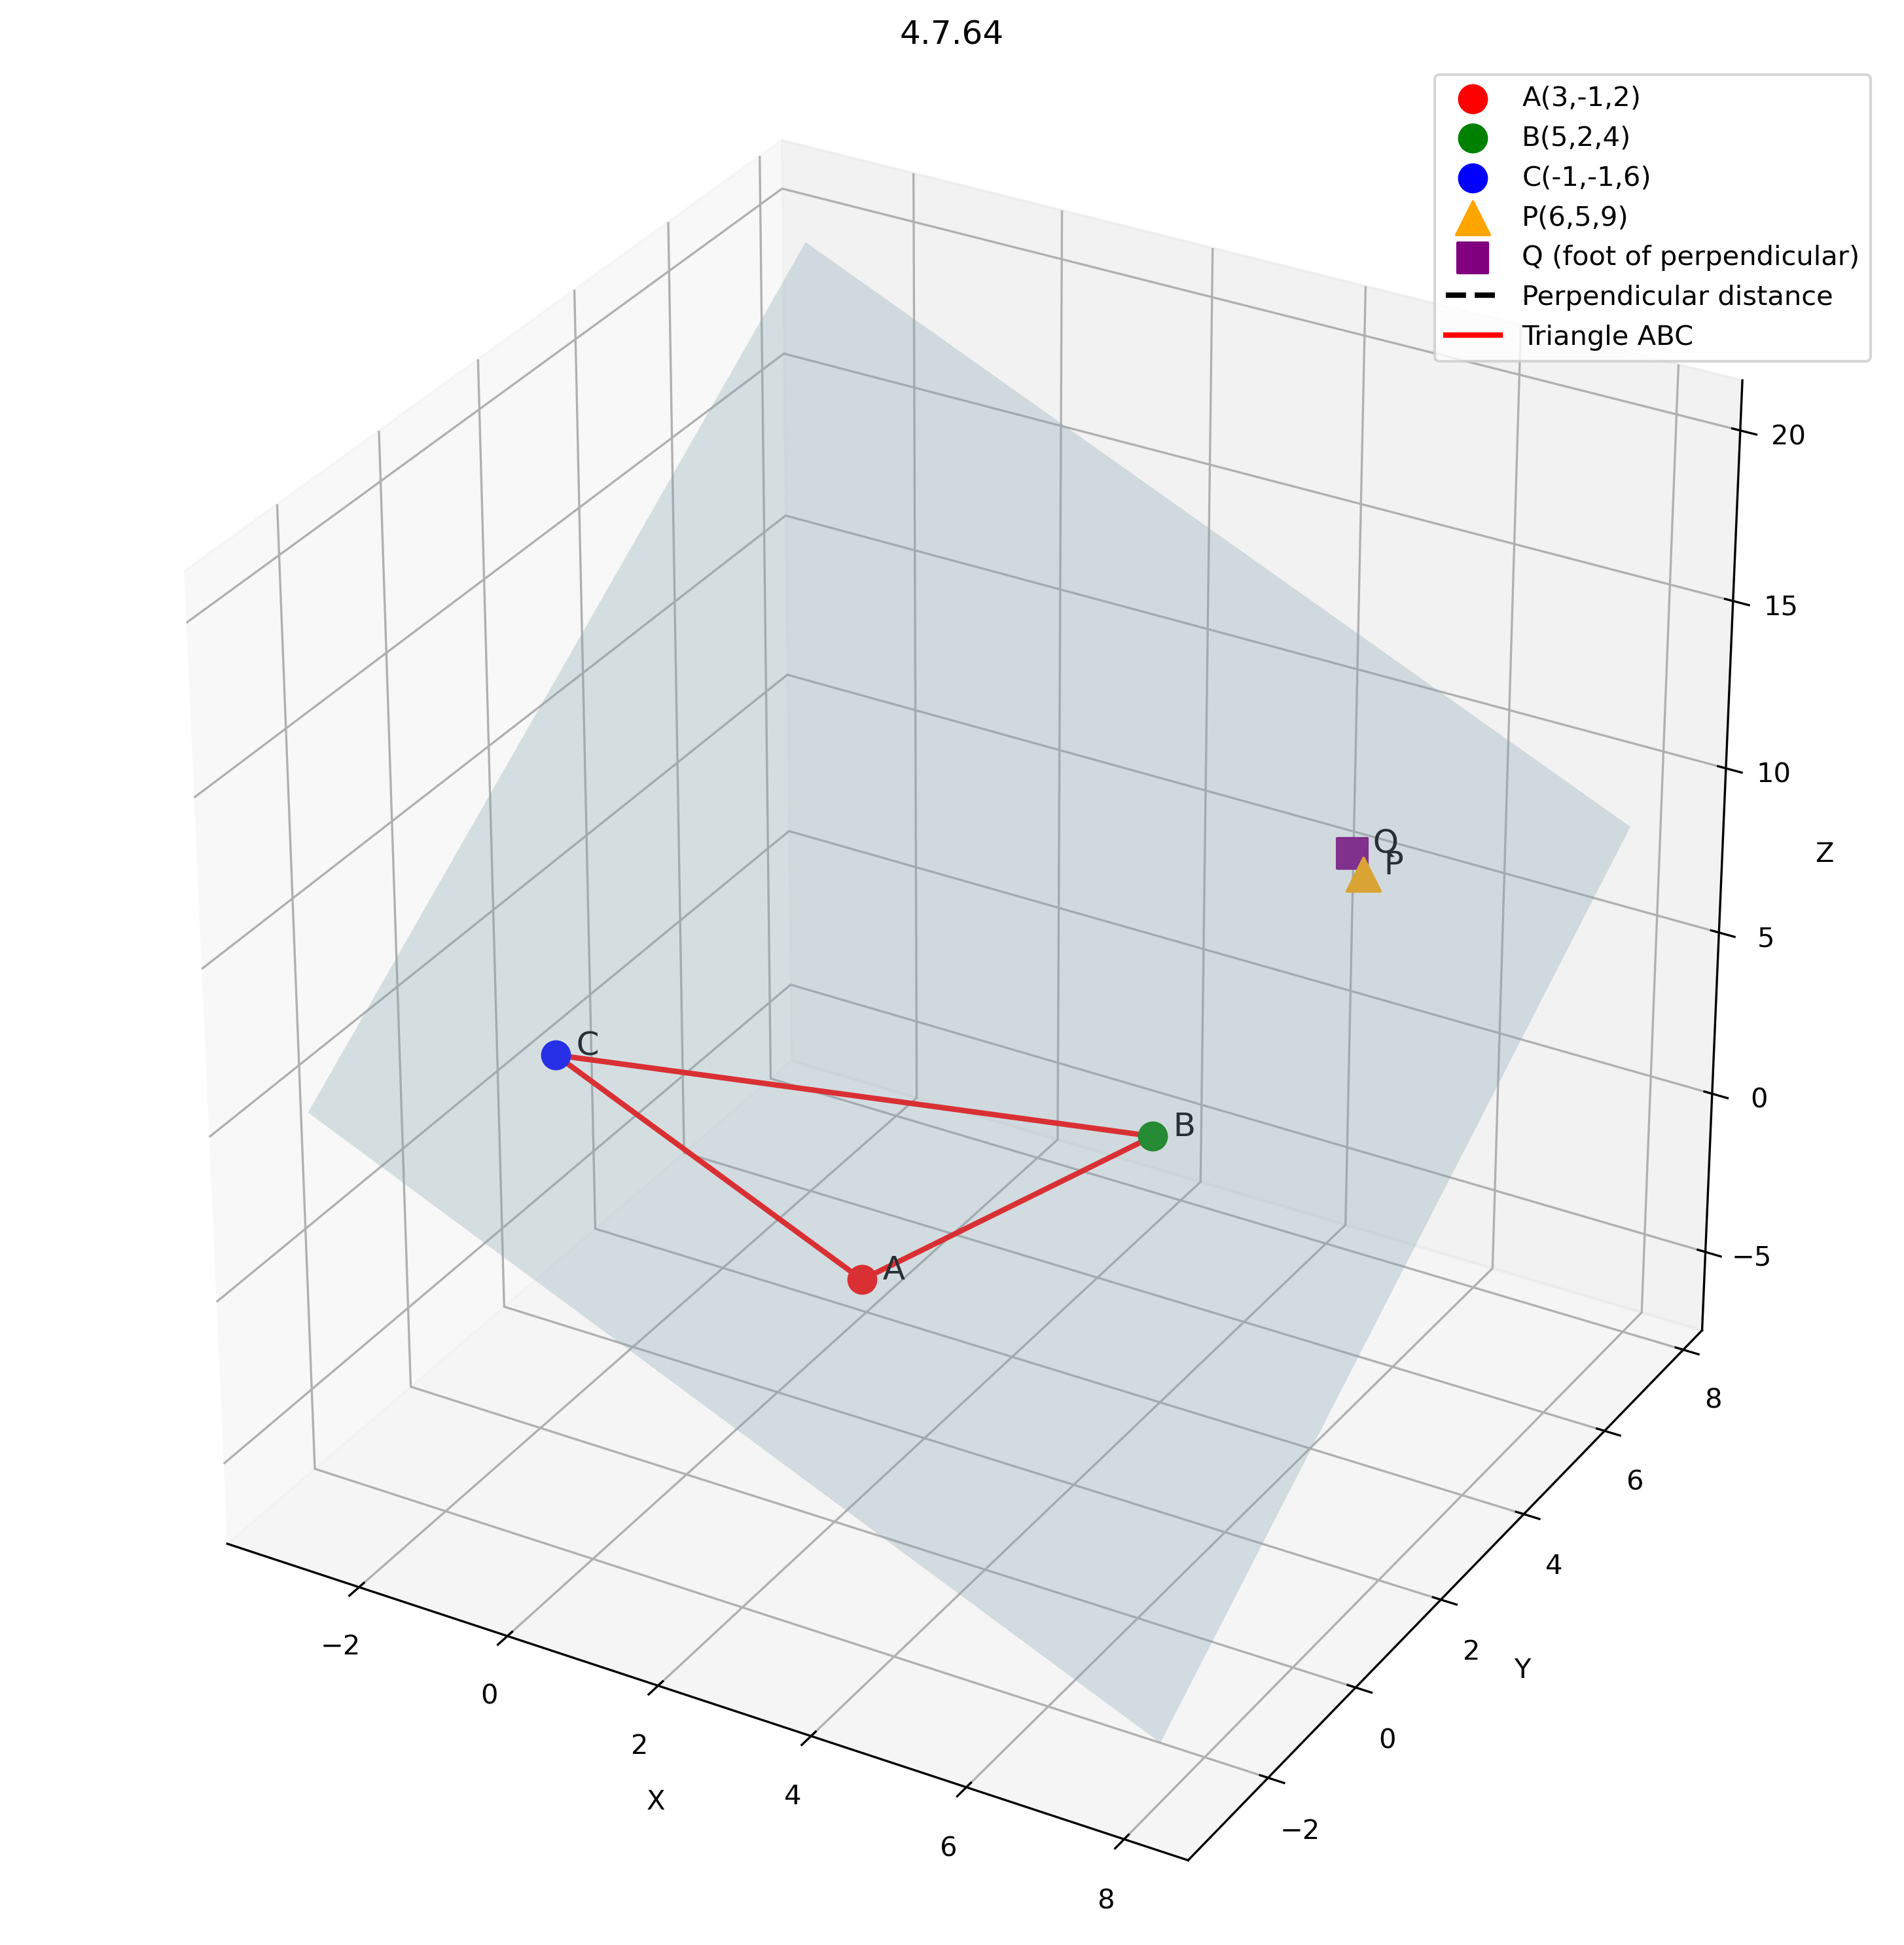
\includegraphics[width=\columnwidth, height=0.8\textheight, keepaspectratio]{figs/fig1.png}
    \label{fig:Beamer/figs/fig1.png}
\end{frame}


\end{document}